%%\graphicspath{{../../figs}}

%% Section
\section{Description of the Methodology Used}

This project has been carried out using a quantitative methodology. This type of methodology is based on the quantification of the results, being the main objective the generation of mathematical models, theories and hypothesis to extract information from an observable phenomena.
Along with the mentioned methodology, a CRISP-DM methodology has been adopted.

\textbf{Cross-industry standard process for data mining}, also known as CRISP-DM, was born in 1996 with the goal of provide a specific methodology suited for the needs of a data mining project. Although this methodology was born with a clear business orientation, it is easy to adapt to the purposes of the work presented here.

The CRISP-DM approach divide the process of data mining in six well differentiated phases shown in the figure \ref{fig:crisp-dm}.
% \cite{wikipedia:crisp-dm_img}.

\begin{figure}[h]
    \centering
    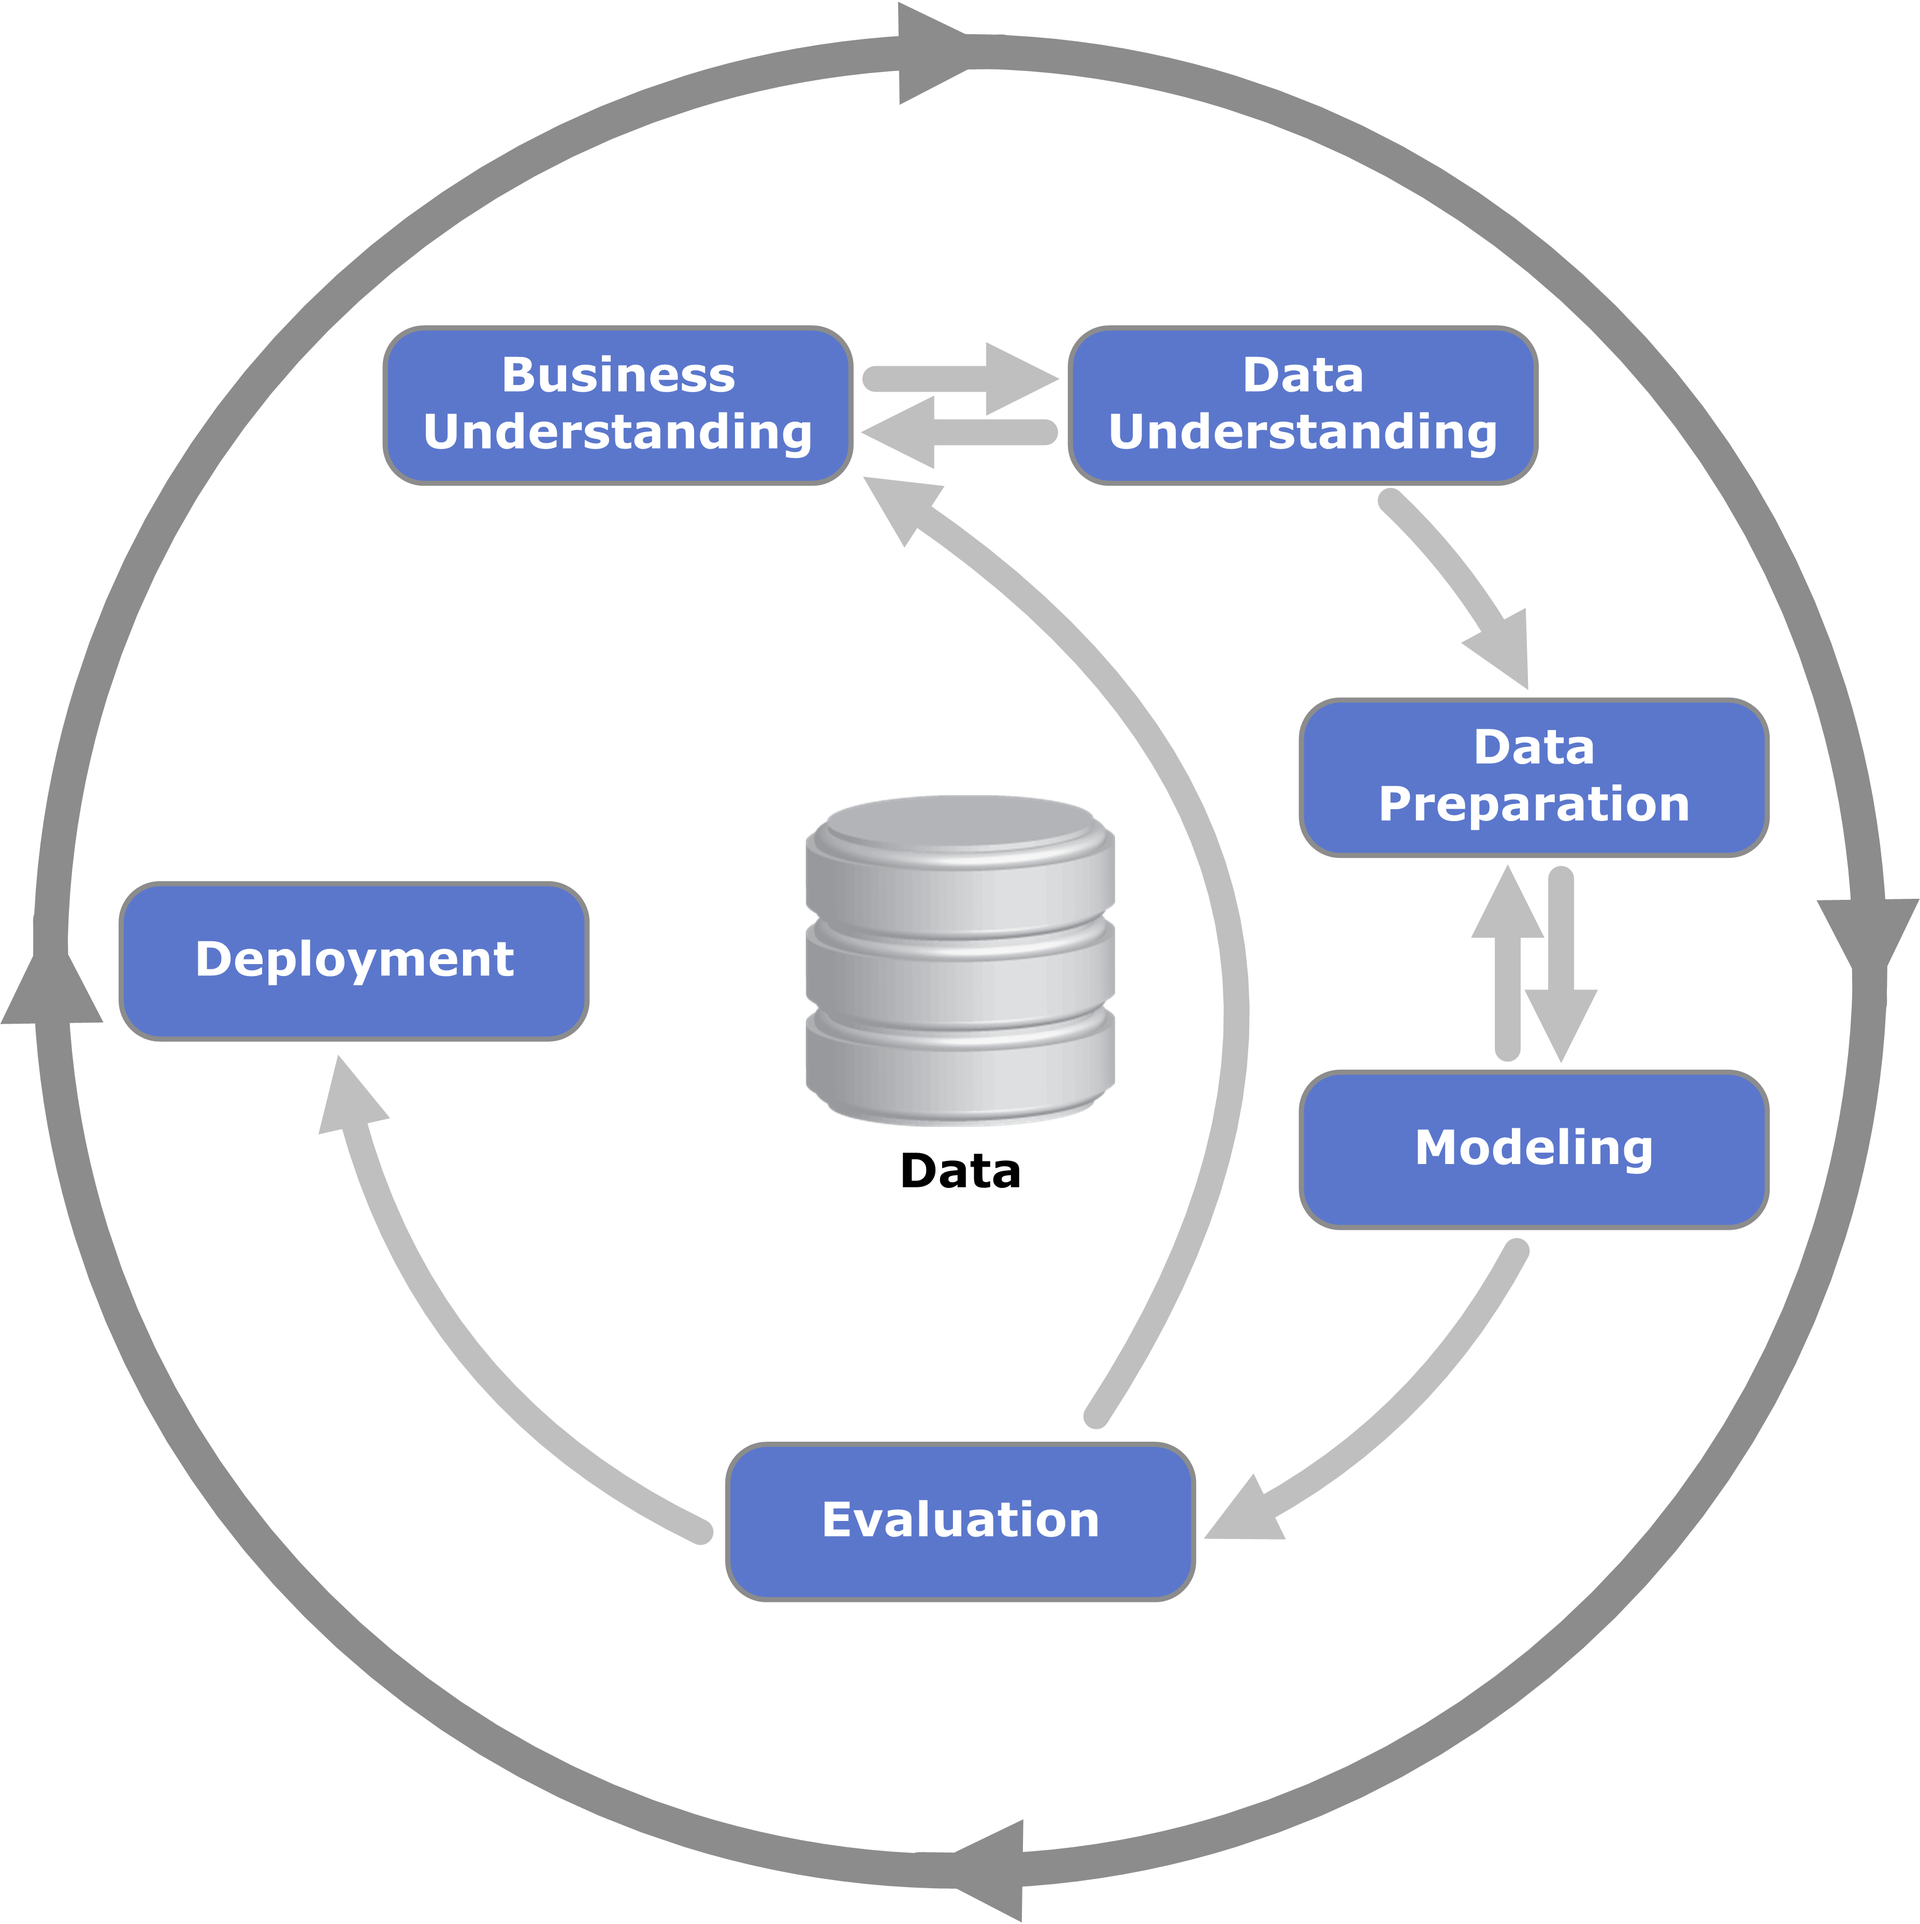
\includegraphics[scale=1]{../figs/CRISP-DM_Process_Diagram.png}
    \caption{CRISP-DM Process diagram by Kenneth Jensen (Own work) [CC BY-SA 3.0 (http://creativecommons.org/licenses/by-sa/3.0)], via Wikimedia Commons.}
    \label{fig:crisp-dm}
\end{figure}

In the following paragraph, a short description of the different phases in the context of this work is provided.

\begin{itemize}
    \item Business Understanding: the main objective in this phase is to understand the problem that is intended to be investigated or solved, set objectives to be accomplished and create a project plan.
    \item Data Understanding: in this phase, the data is collected and explored in order to get familiar with it, understand it or identify possible interesting subsets.
    \item Data Preparation: during this phase, the data is cleaned and transformed if needed in order to produce the final dataset that will be used in the next step.
    \item Modeling: in this phase, modeling techniques are applied in order to obtain a model that allows to give an answer to the initial objectives.
    \item Evaluation: after the generation of the model, an evaluation must be done. During this phase, the model or models obtained in the previous phase are evaluated in order to assess that the results matches the acceptance criteria. After this evaluation is done, it will be possible to analyze the results and extract knowledge from them.
    \item Deployment/Publication: once the results are evaluated and analyzed, the model can be deployed. In the case of being the project a scientific study as in the case of this project, this phase will consist in the publication of the results.
\end{itemize}

An important point to mention here is the iterative nature of the processes. It means that the order of the phases are not fixed, allowing the return to any previous phase in case of necessity.
This point is important in any data mining or machine learning project, but specially in the work presented here, because one key point is the knowledge discovery, and that may require data or specific domain knowledge not contemplated at the early phases of the project.
